\section{Tecnolog\'ias y Herramientas}

\begin{frame}{Tecnolog\'ias y Herramientas}
Inicialmente, se clasifican las herramientas en
tres categor\'ias:

\begin{itemize}
    \item Aplicaciones: herramientas software que permiten al usuario realizar una o
    varias tareas \mbox{espec{\'\i}ficas \cite{GoodwillComputer}}.
    \item Interfaces de Programaci\'on de Aplicaciones (API): interfaces entre una base de c\'odigo y
    el programador \cite{DoucetteOnApi}. Puede verse como como una caja negra
    que provee una determinada funcionalidad.
    \item Librer{\'\i}as/Frameworks: con junto de m\'etodos o funciones a los que se puede invocar.
    En el caso de un framework, incluye tambi\'en patrones de dise\~no
    \mbox{predefinidos \cite{FowlerInversion}}.
\end{itemize}
\end{frame}

\begin{frame}{Tecnolog\'ias y Herramientas (2)}
\framesubtitle{Criterios Generales}
Para poder seleccionar una u otra tecnolog\'ia se plantean los siguientes criterios generales de evaluaci\'on:

\begin{itemize}
   \item Conocimiento t\'ecnico necesario: nivel de conocimiento relativo al \'area necesario para la
   utilizaci\'on de la herramienta. 
   \item Productividad: raz\'on entre las funcionalidades o tareas que pueden
   realizarse utilizando la herramienta y los recursos que toma la implementaci\'on.
   \item Flexibilidad: facilidad de adaptaci\'on de la herramienta para la soluci\'on de diferentes
   tipos de problemas.
\end{itemize}
\end{frame}

\begin{frame}{Tecnolog\'ias y Herramientas (3)}
Además de los criterios mencionados, se consideran criterios espec{\'\i}ficos de cada categor{\'\i}a 
para la evaluaci\'on realizada.
La figura~\ref{figure:esquema-herramientas} muestra un resumen de la clasificaci\'on propuesta. En la parte 
inferior de cada categor\'ia se encuentran ejemplos de
aplicaciones, APIs y librer\'ias respectivamente. 

\begin{figure}[H]
\centering
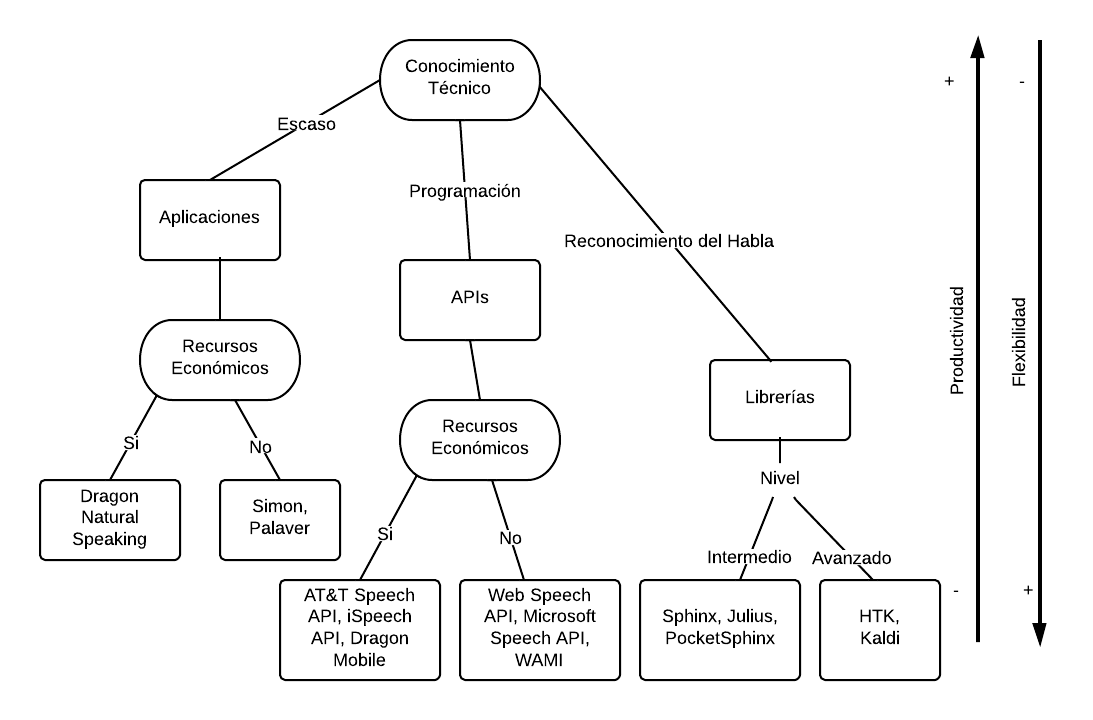
\includegraphics[width=0.8\linewidth]{./graphics/esquema-herramientas.png}
\caption{Esquema de la clasificaci\'on de tecnolog{\'\i}as y herramientas}
\label{figure:esquema-herramientas}
\end{figure}
\end{frame}
